\begin{figure}[!]
    \begin{subfigure}{\textwidth}
    \centering
    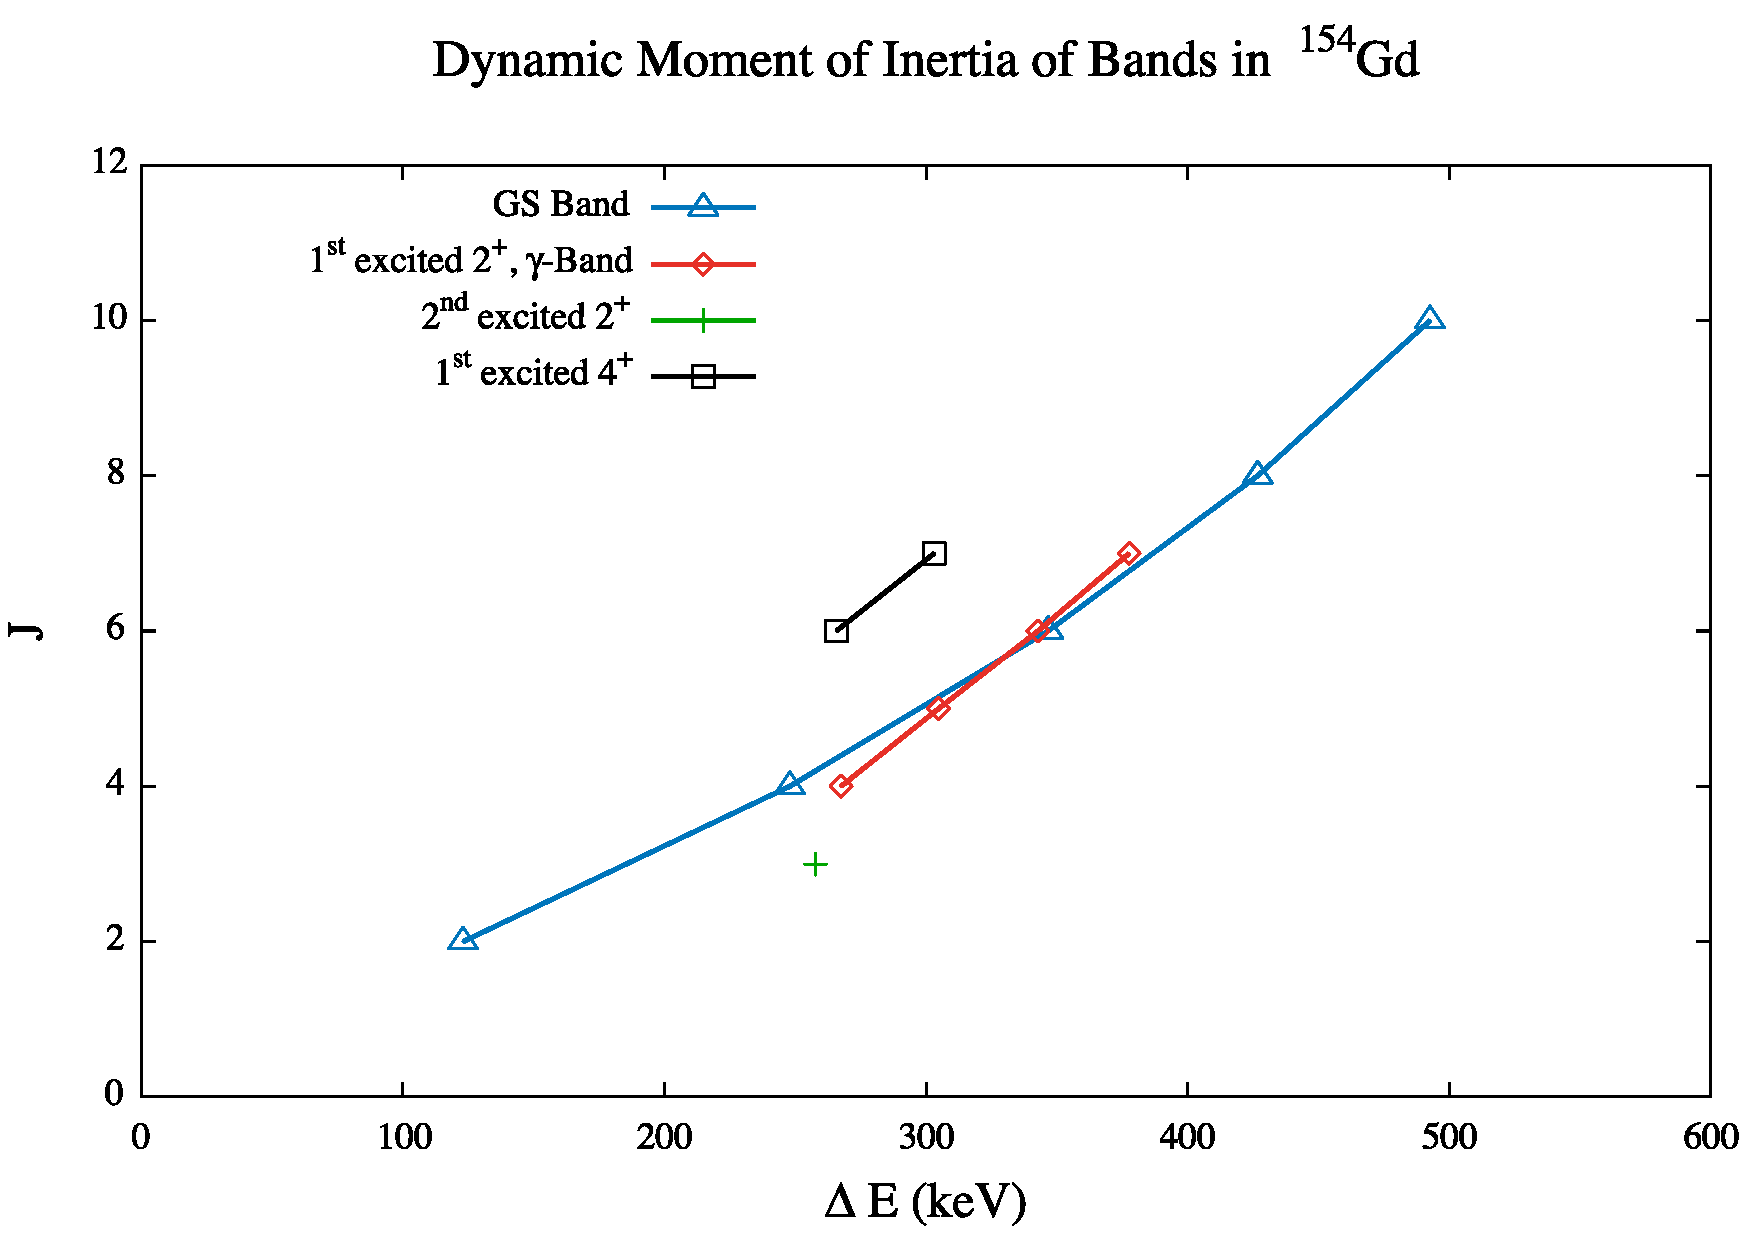
\includegraphics[scale=0.4]{Discussion/154_Dynamic.pdf}
    \caption*{(a)}
    \end{subfigure}
    \begin{subfigure}{\textwidth}
    \centering
    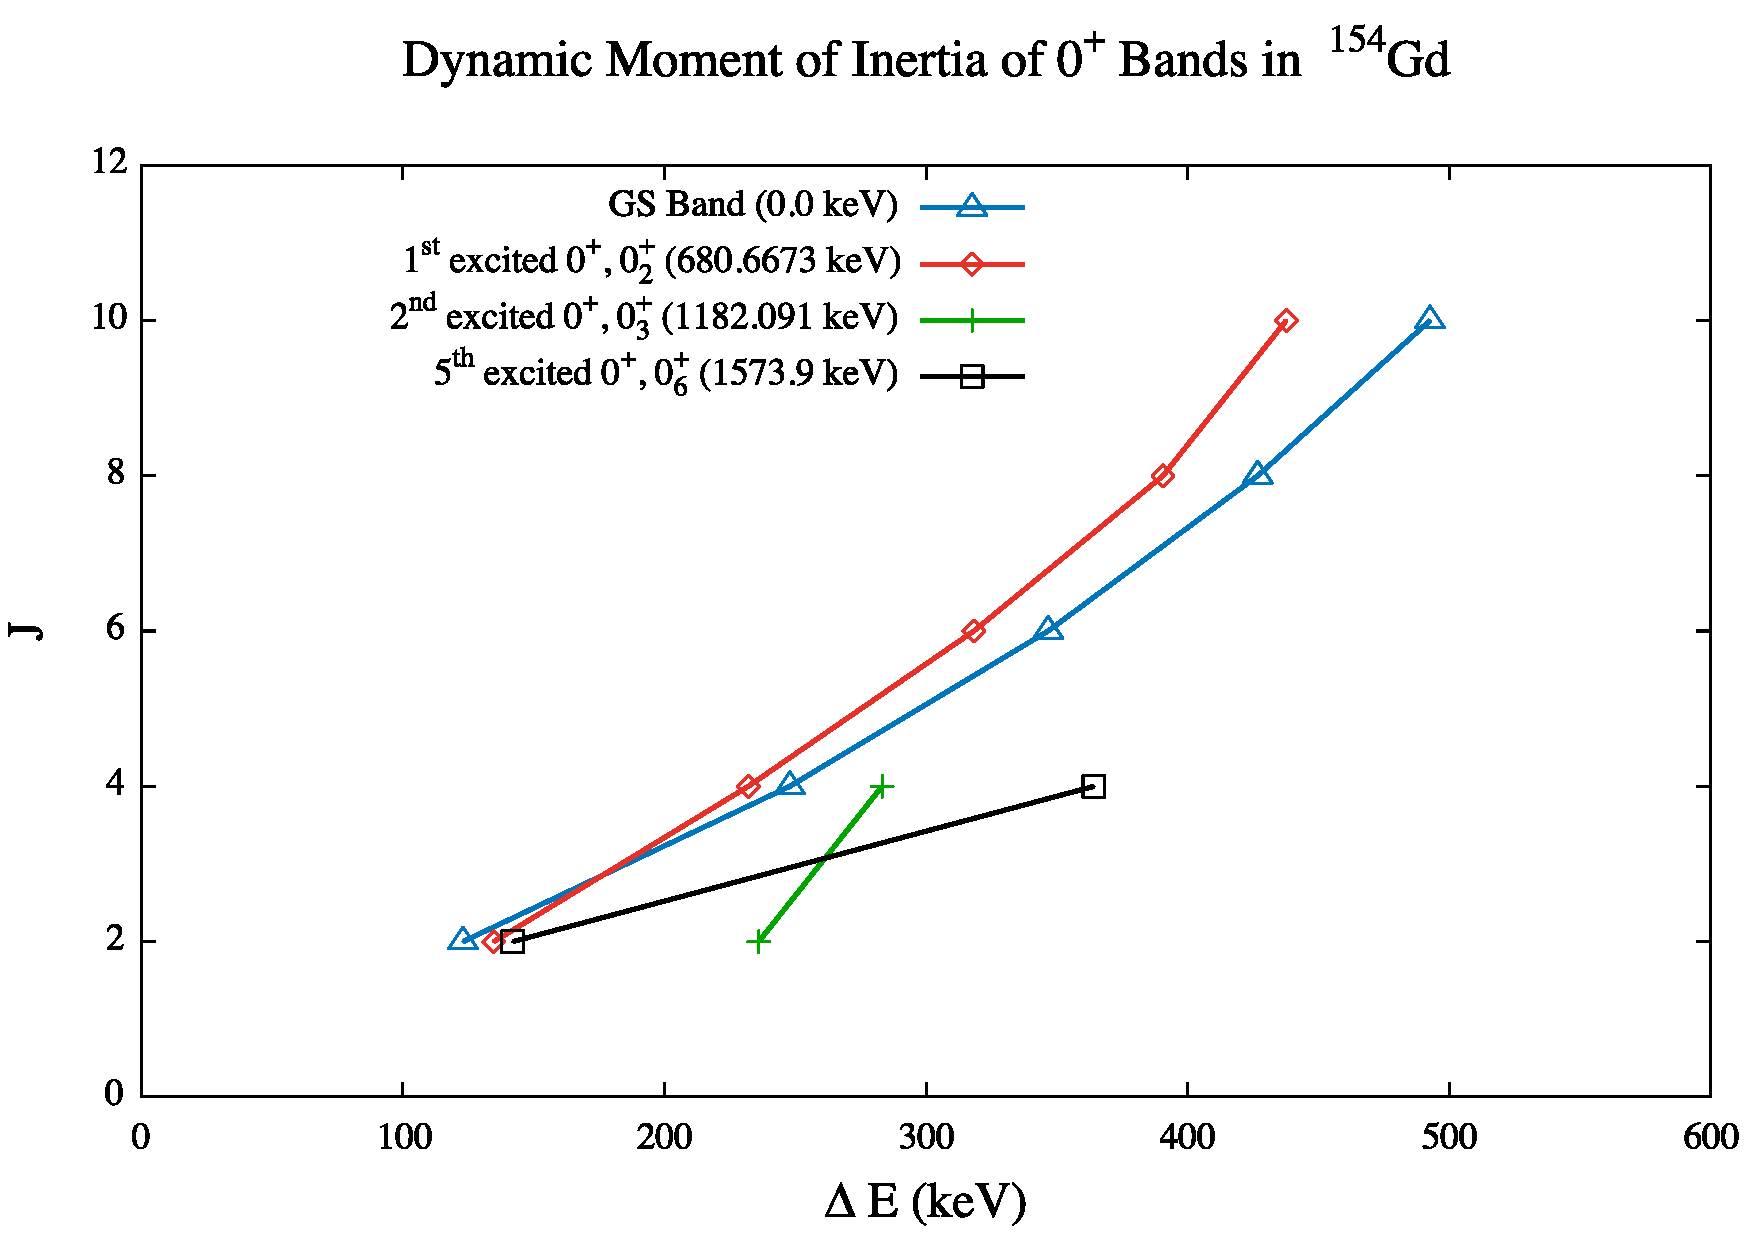
\includegraphics[scale=0.4]{Discussion/154_Dynamic0.pdf}
    \caption*{(b)}
    \end{subfigure}
    \caption{(a) The dynamic moments of inertia of the ground state, $K=2^+_1$ and $K=4^+_1$ bands. As is seen visually and with the slopes, the ground state band and the $\gamma$ band have similar moments of inertia and the $K=2^+_1$ and $K=4^+_1$ bands have identical moments of inertia. (b) The dynamic moments of inertia of the four $0^+$ bands seen in the experiment. The ground state band and the first excited $0^+$ band have very similar moments of inertia, while the second and fifth $0^+$ bands differ greatly.}
    \label{fig:154_Dynamic}
\end{figure}